\setchapterimage[3cm]{seaside}
\chapter{Model description}
\label{Chapter2} % For referencing the chapter elsewhere, use \ref{Chapter2} 
\section{H transport} \label{description_H_transport_model}
\subsection{Bulk model}
As in most of MRE models, HIs are split in several populations which are the mobile and the trapped ones in the i-th trap, described using their concentration (respectively $c_\mathrm{m}$ and $c_{\mathrm{t},i}$).
The spatio temporal evolution of these concentrations are commonly described by the following reaction-diffusion system:

\begin{equation}
    \frac{\partial c_\mathrm{m}}{\partial t}=\vec{\nabla} \cdot\left(D(T) \vec{\nabla}c_\mathrm{m}\right)+\Gamma-\sum \frac{\partial c_{\mathrm{t}, i}}{\partial t}
    \label{eq:mobile}
\end{equation}

\begin{equation}
    \frac{\partial c_{\mathrm{t}, i}}{\partial t}=k(T) \cdot c_\mathrm{m} \cdot\left(n_{i}-c_{\mathrm{t}, i}\right)-p(T) \cdot c_{\mathrm{t}, i}
    \label{eq:trapped}
\end{equation}

In Equation \ref{eq:mobile}, ${D(T)=D_0 \exp\big(\frac{-E_\mathrm{D}}{k_B \cdot T}\big)}$ is the diffusion coefficient in \si{m^2.s^{-1}}, $T$ being the temperature in $\si{K}$ and ${k_B = 8.617 \times 10^{-5} \si{eV.K^{-1}}}$ the Boltzmann constant, $\Gamma$ is the volumetric source term of particles in \si{m^{-3}.s^{-1}}, $k(T)=k_0\exp{\big(\frac{-E_{k, i}}{k_B \cdot T}\big)}$ and $p(T)=p_0\exp{\big(\frac{-E_{p, i}}{k_B \cdot T}\big)}$ are the trapping and detrapping rates expressed in \si{m^3.s^{-1}} and \si{s^{-1}} respectively and $n_i$ is the trap density in \si{m^{-3}}.
The unit of the different concentration, $c_\mathrm{m}$ and $c_{\mathrm{t},i}$ are in $ \si{m^{-3}}$ but can be expressed in atomic fraction (at.fr.) by normalising them to the atomic density of the material.
\subsection{Boundary conditions}

Several boundary conditions will be employed in order to constrain either the actual solution (Dirichlet) or the solution gradient (Neumann, Robin) at the domain's boundaries.

\subsubsection{Dirichlet boundary conditions}

Concentration can be fixed at the surface by applying Dirichlet boundary conditions as described in Equation \ref{eq:dirichlet bc}.
\begin{equation}
    c_\mathrm{m} = c_0(x, t) \quad \text { on } \partial \Omega
    \label{eq:dirichlet bc}
\end{equation}
where $\partial \Omega$ is the domain boundary.

$c_0$ can be calculated from Sievert's law of equilibrium and Equation \ref{eq:dirichlet bc} reads:
\begin{equation}
    c_\mathrm{m} = S(T) \sqrt{P}\quad \text { on } \partial \Omega
\end{equation}
where $P$ is the partial pressure of hydrogen at the boundary in \si{Pa}, $S(T)=S_0 \exp(\frac{-E_S}{k_B T})$ is the material solubility in \si{m^{-3}.Pa^{-1/2}} and $T$ is the local temperature in \si{K}.
This law of equilibrium is a steady-state approximation of a more complex model which takes into account flux exchanges between adsorbed and mobile concentrations at the boundary.
It is therefore valid when applied to cases where the kinetics is slow enough for the system to remain at equilibrium.

\subsubsection{Neumann \& Robin boundary conditions}

Concentration gradient can also be constrained on the boundaries as described in Equation \ref{eq: neuman robin bc}.

\begin{equation}
    D(T)\nabla c_\mathrm{m} = f(x, t) \quad \text { on } \partial \Omega
    \label{eq: neuman robin bc}
\end{equation}
where $D(T) = D_0 \exp(\frac{-E_D}{k_B T}) $ is the diffusion coefficient in \si{m^2.s^{-1}}, $T$ is the local temperature in \si{K} and $\partial \Omega$ is the domain boundary.

$f$ can be expressed as a molecular recombination flux and Equation \ref{eq: neuman robin bc} reads:
\begin{equation}
    D(T)\nabla c_\mathrm{m} = K_r(T) c_\mathrm{m}^n \quad \text { on } \partial \Omega
\end{equation}
where $K_r(T) = K_{r_0} \exp(\frac{-E_{K_r}}{k_B T}) $ is the recombination coefficient expressed in \si{m^{3n-2}.s^{-1}} and $n \in \{1, 2\}$ is the order of the recombination.


\subsubsection{Analytical simplification}
Assuming a narrow Gaussian distribution for the source term $\varphi_\mathrm{imp}$, the mobile particles concentration profile can be approximated \textcolor{black}{by a triangular shape\cite{schmid_diffusion-trapping_2016} (see Supplementary Figure \ref{fig:recomb sketch})}.

\begin{figure*}[h!]
    \centering
    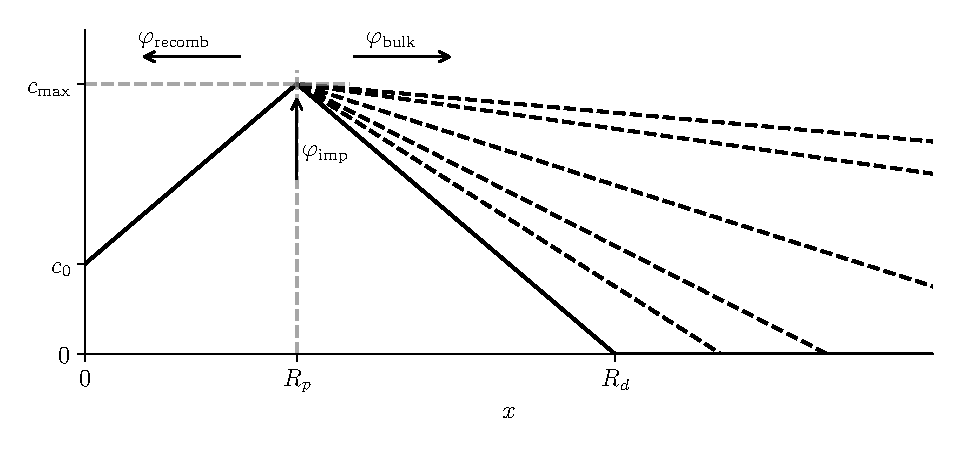
\includegraphics[width=0.75\linewidth]{Figures/Chapter2/recomb_sketch.pdf}
    \caption{Concentration profile with recombination flux and volumetric source term at $x=R_p$. Dashed lines correspond to time evolution.}
    \label{fig:recomb sketch}
\end{figure*}

The expression of $c_\mathrm{max}$ can be obtained by expressing the flux balance at equilibrium:

\begin{equation}
    \varphi_\mathrm{imp} = -\varphi_\mathrm{recomb} + \varphi_\mathrm{bulk}
    \label{eq:flux balance}
\end{equation}
where $\varphi_\mathrm{recombination}$ is the recombination flux and $\varphi_\mathrm{bulk}$ is the migration flux.

$\varphi_\mathrm{bulk}$ can be expressed as:
\begin{equation}
    \varphi_\mathrm{bulk} = D \cdot \frac{c_\mathrm{max}}{R_d(t) - R_p}
\end{equation}

When $t \rightarrow \infty$ or $R_d \gg R_p$ (a ratio of 10 or 100 is enough), $\varphi_\mathrm{bulk} \ll \varphi_\mathrm{recomb}$.
According to Fick's law, Equation \ref{eq:flux balance} reads:

\begin{eqnarray}
    \varphi_\mathrm{imp} &= D \cdot \frac{c_\mathrm{max}-c_{0}}{R_{p}} \\
    \Leftrightarrow c_\mathrm{max} &= \frac{\varphi_\mathrm{imp} R_{p}}{D}+ c_0
    \label{eq:c_max}
\end{eqnarray}

Equation \ref{eq:flux balance} can also be written by expressing $\varphi_\mathrm{recombination}$ as a function of the recombination coefficient $K$:

\begin{eqnarray}
    \varphi_\mathrm{imp} &= K c_{0}^{2} \\
    \Leftrightarrow c_{0} &= \sqrt{\frac{\varphi_\mathrm{imp}}{K}}
    \label{eq:c_0}
\end{eqnarray}

By replacing Equation \ref{eq:c_0} in Equation \ref{eq:c_max} one can obtain:

\begin{equation}
    c_\mathrm{max} = \frac{\varphi_\mathrm{imp} R_{p}}{D}+\sqrt{\frac{\varphi_\mathrm{imp}}{K}}
\end{equation}

As the recombination process becomes fast (\textit{ie} $K \rightarrow \infty$), $c_0 \approx 0$ and $c_\mathrm{max} \approx \frac{\varphi_\mathrm{imp} R_{p}}{D}$.


\subsection{Interface conditions}
According to \sidecite{krom_hydrogen_2000} since the solubility of hydrogen atoms in solids is low, the chemical potential of solute hydrogen $\mu$ is expressed by:
\begin{equation}
    \mu = \mu_0 + RT \ln\left( \frac{c_\mathrm{m}}{N_L}\right)
\end{equation}
where $\mu_0$ is the chemical potential in a reference state in \si{J.mol^{-1}}, $R$ the ideal gas constant, $T$ the temperature in \si{K}, $c_\mathrm{m}$ the mobile hydrogen concentration in \si{m^{-3}} and $N_L$ the lattice site concentration in \si{m^{-3}}.

Assuming that only free hydrogen atoms contribute to the overall flux in the material, the particle flux $J$ in \si{m^{-2}.s^{-1}} can be expressed by Fick's law:
\begin{equation}
    J = - D \nabla c_\mathrm{m}
\end{equation}
where $D$ is the diffusion coefficient of hydrogen in a non-stress lattice expressed in \si{m^{2}.s^{-1}}. 


%The temporal evolution of hydrogen concentration in materials is governed by Fick's law of diffusion (see Equation \ref{eq:diffusion equation}).

%\begin{equation}
%    \frac{\partial c}{\partial t}=\vec{\nabla} \cdot\left(D \vec{\nabla}c\right)+ f
%    \label{eq:diffusion equation}
%\end{equation}
%where $c$ is the hydrogen concentration in \si{m^{-3}}, D is the diffusion coefficient of the mobile hydrogen in the material in \si{m^2.s^{-1}} and $f$ is the source term in \si{m^{-3}.s^{-1}}.

%In order to take into account the conservation of chemical potential across an interface, one must not ensure concentration continuity but rather the continuity of the chemical potential of the species in the material.

%The chemical potential is expressed  expressed in \si{J.mol^{-1}} as follow: \textcolor{red}{YC-> pas sûr qu'il faille garder cette equation ma foi...}
%\begin{equation}
%    \mu = \mu_0 + RT\ln{\left(\frac{c}{S} \frac{1}{p_0}\right)}
%\end{equation}
%where $\mu_0$ is the species standard chemical potential, $R$ is the gas constant expressed in \si{J.K^{-1}.mol^{-1}}, $T$ is the temperature in \si{K}, $S$ is the solubility of the species in the material expressed in \si{m^{-3}.Pa^{-0.5}} and $p_0$ is the pressure in \si{Pa} at some reference state.

%It can be shown that the continuity of $\mu$ is equivalent to that of $c/S$ \sidecite{}.
The local equilibrium at the interface between two materials must ensure  the continuity of both the chemical potential $\mu$ (see Equation \ref{eq: muconservation}) and the particle flux (see Equation \ref{eq: flux conservation}).
\begin{equation}
            \mu^- = \mu^+  \label{eq: muconservation}  
\end{equation}
    
\begin{equation}
        D^- \nabla c_\mathrm{m}^- = D^+ \nabla c_\mathrm{m}^+ \label{eq: flux conservation} 
\end{equation}
The chemical potential continuity can also be ensured by the continuity of the quantity $c_\mathrm{m}/S$ (see Equation \ref{eq: c/s conservation}) for mechanical stress-free materials in thermodynamic equilibrium and the Soret effect being neglected:
\begin{equation}
                \left(\frac{c_\mathrm{m}}{S}\right)^- = \left(\frac{c_\mathrm{m}}{S}\right)^+  \label{eq: c/s conservation}  
\end{equation}
Here, the quantity $c_\mathrm{m}/S$, with $S$ the solubility of hydrogen expressed in \si{m^{-3}.Pa^{-0.5}}, is equivalent to the root square of the pressure of an imaginary gas in thermodynamic equilibrium between the two solids and for which Sievert's law is applied.  
% Ref annex B
This assumption is correct as long as the time needed to reach the equilibrium is low compared to the time of the simulation.
\ref{appendix transient model} described the characteristic time calculated by a transient interface model.
For long exposure time (as in Section \ref{iter case}) as well as for high temperatures, it is shown that the characteristic time is small enough for the equilibrium model to be valid.

From Equation \ref{eq: c/s conservation}, one can deduce that a solubility discontinuity across an interface induces a discontinuity of mobile hydrogen concentration $c_\mathrm{m}$.
This can also be interpreted as the chemical potentials at a reference state being different in different materials \sidecite{kirchheim_25_2014}, as the lattice site concentration.

% To ensure a correct treatment of the material interface in hydrogen transport codes, two approaches can be used.
% The most natural is to solve the hydrogen mobile concentration transport in both materials (see Equation \ref{eq: diffusion equation}) and impose an internal condition at the interface between the two materials to verify Equation \ref{eq: c/s conservation} \sidecite{longhurst_tmap7_2008}.
% The other way is to apply a change of variable in the hydrogen transport equation with $\phi = c_\mathrm{m}/S$ (see Equation \ref{eq: diffusion equation changed})  \sidecite{smith_abaqusstandard_2009} when internal boundary can not be defined. Because $\phi$ is solved, the ratio $c_\mathrm{m}/S$ is continuous by default at the material interfaces.

To ensure a correct treatment of the material interface in hydrogen transport codes, two approaches can be employed.
The most straightforward approach is to solve the hydrogen mobile concentration transport in both materials (see Equation \ref{eq: diffusion equation}) and enforce the concentration jump at the interface between the two materials with an internal condition verifying  Equation \ref{eq: c/s conservation} \sidecite{longhurst_tmap7_2008}.

\begin{equation}
    \frac{\partial c_\mathrm{m}}{\partial t}=\nabla \cdot\left(D \nabla c_\mathrm{m}\right) + f
   \label{eq: diffusion equation}
\end{equation}
where $f$ is the source term in \si{m^{-3}.s^{-1}}.

Another method is to perform a change of variable in Fick's second law of diffusion with $\phi = c_\mathrm{m}/S$ \sidecite{smith_abaqusstandard_2009} when internal conditions cannot be set.
Equation \ref{eq: diffusion equation} therefore reads:

\begin{align}
    \frac{\partial \phi S}{\partial t} &= \nabla \cdot\left(D \nabla \phi S\right) + f \nonumber \\
    &=\nabla \cdot\left( D S \nabla \phi + D \phi \nabla S\right) + f \label{eq: diffusion equation changed}
\end{align}

Because $\phi$ is computed, the ratio $c_\mathrm{m}/S$ is continuous by default at the material interfaces.

This second approach is used for instance in the \textit{mass-diffusion} procedure of the Abaqus code.
However, this procedure cannot be directly used to simulate hydrogen transport with thermomechanical loading \textit{(coupled temperature displacement} procedure) \sidecite{smith_abaqusstandard_2009}.
Indeed, the \textit{mass-diffusion} procedure can solve mechanically-assisted diffusion problems, knowing the spatio-temporal evolution of the mechanical pressure.
The \textit{temperature-displacement} procedure is used to simultaneously solve diffusion and mechanical problems.
To account for both mechanical fields, trapping influence on diffusion and transient heat transfer, User Subroutines are employed.
\ref{appendix abaqus} describes the implementation based on user Subroutines.
This interface model has also been implemented into the current hydrogen transport code FESTIM \sidecite{delaporte-mathurin_finite_2019} using FEniCS \sidecite{alnaes_fenics_2015}.


\section{Heat transfer}
\subsection{Bulk model}

The heat equation is described as follow:
\begin{equation}
    \rho \cdot C_p \frac{\partial T}{\partial t}=\nabla \cdot (\lambda \nabla T)
    \label{eq:heat equation}
\end{equation}
where $\rho$ is the density of the material in \si{kg.m^{-3}}, $C_p$ its specific heat capacity expressed in \si{J.kg^{-1}.K^{-1}} and $\lambda$ the thermal conductivity expressed in \si{W.K^{-1}}.

\subsection{Boundary conditions}
\section{Summary}